\chapter{Cosmology with the 21\ cm Line}
\label{ch1}

Early on in cosmic history, the universe was extremely hot and dense.  
Cosmic expansion caused the universe to cool, 
eventually reaching temperatures where the first atoms (principally hydrogen) could become neutral,
i.e., protons and electrons combined into neutral hydrogen.
For a long period afterwards, known as the ``cosmic dark ages," the universe was very simple;
small density perturbations in the cosmic matter field (consisting of both dark
and ordinary or ``baryonic" matter), however, grew through gravitational collapse:
overdense regions exerted a stronger gravitational pull on their surroundings, attracting even more
matter and growing even denser.  Eventually, some perturbations became dense enough for
nuclear fusion to begin, leading to the formation of the first stars, and eventually, galaxies.  
Our research seeks to understand this ``cosmic dawn": 
the formation of the first luminous objects in the universe.

\section{Reionization}

Of particular interest is the era known as the Epoch of Reionization (EoR).
This period occurs at the late stages of cosmic dawn, when the first galaxies became
numerous enough to output a substantial number of ultraviolet photons into
intergalactic space.
These photons are energetic enough to cause the ``reionization" of hydrogen, which had
been neutral since the early universe.
The exact timing of the EoR is still unknown, but theories predict it occurred
500 million years after the Big Bang, corresponding to a redshift of $z \sim 6-12$.

In many ways, the EoR forms the bridge
between the fundamental physics and cosmology of the early universe
and the complicated astrophysics of galaxy formation.  As such, measurements
of the conditions during the EoR promise a wealth of information about
the evolution of structure in the universe.  Detailed reviews of the
EoR can be found in \cite{furlanetto_et_al_2006} and 
\cite{barkana_and_loeb_2007}, as well as in the textbooks of
\cite{loeb_and_furlanetto_2013} and \cite{mesinger_2016}.

\section{The 21\ cm Line}

Observational studies of the Epoch of Reionization are difficult; the first galaxies are distant and small,
and therefore cannot be detected by current telescopes.  (The James Webb Space Telescope may see some
of the very largest galaxies during the EoR, but cannot detect more ``typical members" of the galaxy population.)
Our research pioneers a new technique that offers a potentially unparalleled view into the physics of the EoR.
This technique is often referred to as ``21\ cm cosmology."
Detailed reviews of this field can be found in \cite{furlanetto_et_al_2006},
\cite{morales_and_wyithe_2011}, and \cite{pritchard_and_loeb_2012}.

The so-called 21\ cm transition is the hyperfine spin-flip transition
of neutral hydrogen; that is to say, the energy difference between 
the aligned and anti-aligned states of the proton and electron in a hydrogen atom
is $5.9\times10^{-6}$~eV, corresponding to a photon of wavelength 21\ cm.
Although the lifetime of the excited state is exceedingly long ($\sim10^7$ years),
the high abundance of neutral hydrogen in the universe is more than enough
to compensate for the long lifetime and make the transition observable.
Moreover, the weakness of the line guarantees that it is always
optically thin in all but the most extreme systems.  Therefore, the principal
idea of 21\ cm cosmology is relatively simple: observe all the neutral hydrogen
in the universe.  At cosmological distances, the observed frequency of
the 21\ cm emission can easily be mapped into a distance, with the redshifting
caused by cosmic expansion.  The ultimate promise of 21\ cm cosmology
is thus a 3-dimensional map of the distribution of neutral hydrogen in the
universe.

Observations of the 21\ cm line during the EoR offer a unique view into this era.
Rather than trying to observe the first galaxies themselves, we seek to observe emission
from intergalactic hydrogen.  As reionization proceeds, more and more hydrogen in the
intergalactic medium (IGM) becomes ionized and stops emitting 21\ cm radiation.
By observing the spatial distribution of the ionized ``bubbles" around the first galaxies,
and their growth as a function of redshift, we can glean information about the galaxies themselves.
The left hand side of Figure \ref{fig:cubes_and_pspecs} shows four redshift slices from a simulation of reionization.
Ionized bubbles (shown in red) are seen to grow around the first galaxies, eventually overlapping at late times.
At $z \lesssim 6$, the intergalactic medium is expected to be completely ionized.
\begin{figure}[htbp!]
\centering
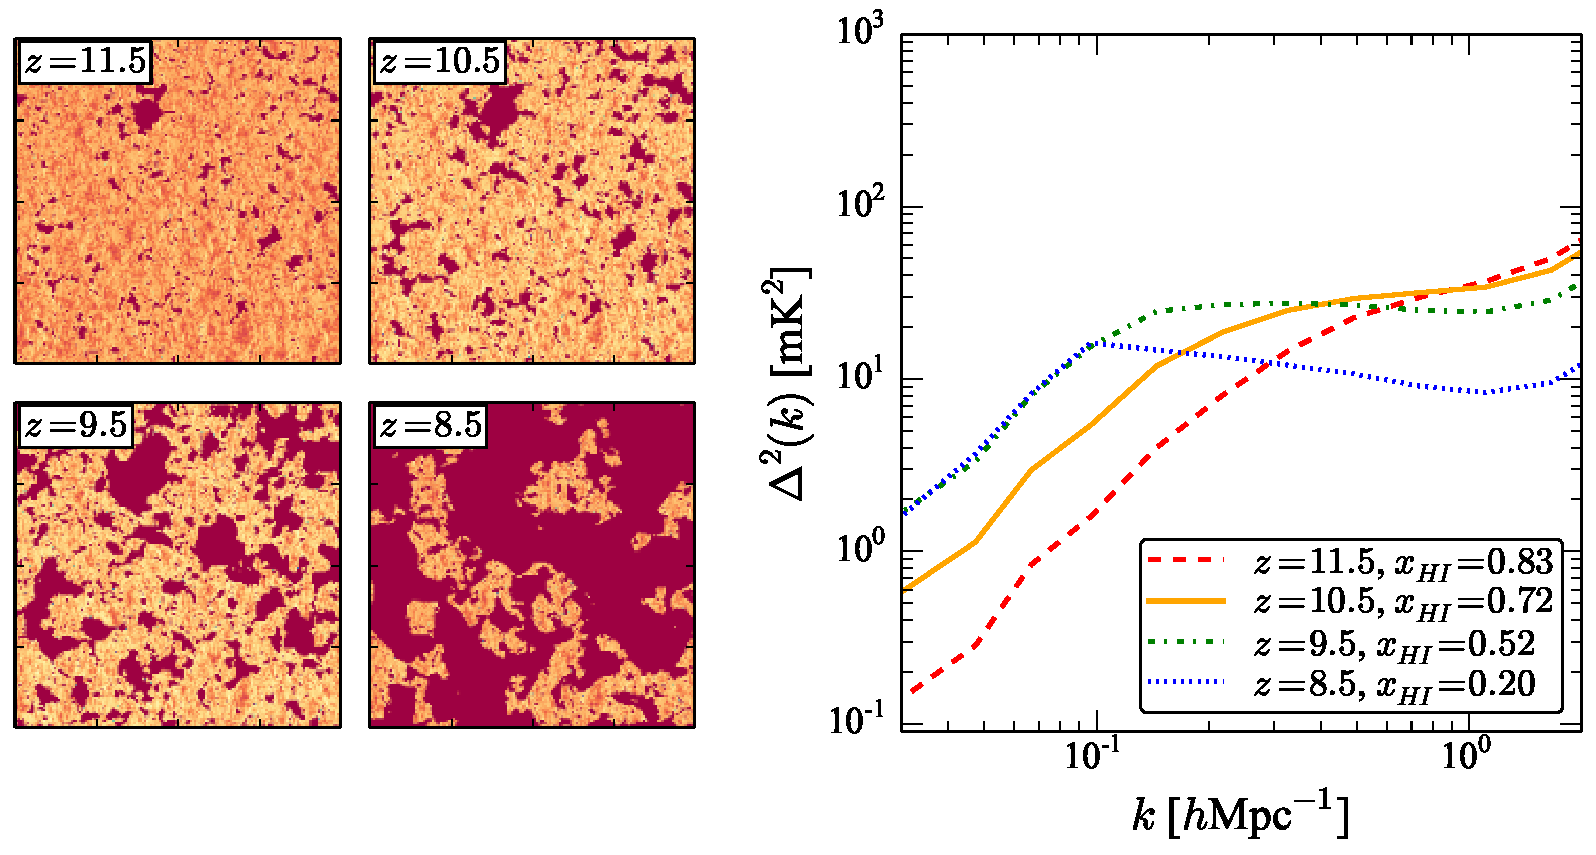
\includegraphics[width=4.5in]{figures/cubesAndPspecs.pdf}
\caption{\emph{Left}: Slices of a 21\ cm signal simulation at 4 different redshifts.  Ionized bubbles, shown in red, grow around the first galaxies as time progresses (i.e. as redshift, $z$, decreases).  \emph{Right}: The corresponding power spectra for the four redshifts on the left; $x_{\rm HI}$ refers to the total fraction of the universe that is neutral at that redshift.}
\label{fig:cubes_and_pspecs}
\end{figure}
Since we probe the \emph{cumulative} effect of all the ionizing photons emitted into the IGM,
21\ cm cosmology probes the more numerous and more typical small galaxies that are unobservable through
any other means.

\section{Power Spectra}

As we shall see in chapter \ref{ch2}, our current 21\ cm cosmology experiments do not have the
sensitivity or angular resolution to actually image the bubbles during the reionization
epoch.  Until larger instruments are constructed, we must target a \emph{statistical} detection of these
features, and study the evolution of this statistical signal in order to glean cosmological information.
Our current statistic of choice is known as the \emph{power spectrum}.  The power spectrum
measures the amount of signal as a function of scale quantified through Fourier space $k$-modes.
Small $k$ modes probe signal on large scales, and large $k$ modes probe signal on small scales.
The right hand side of Figure \ref{fig:cubes_and_pspecs} shows the power spectra corresponding to the
simulated redshift slices shown on the left.  As reionization proceeds, more power moves to large scales (i.e. small values
of $k$) because the bubbles grow bigger.  Typically, when the universe is 50\% neutral ($x_{\rm HI} = 0.5$), the
21\ cm power spectrum is expected to be largest.

\section{Foregrounds}

No one has yet detected the 21\ cm signal from the EoR.  This is principally due to the presence of bright
\emph{foreground} emission, i.e., other radio signals between us and the signal from cosmological hydrogen.
The brightest foregrounds are emission from other galaxies as well as the Milky Way itself.  Taken together, 
these sources are approximately five orders of magnitude brighter than the 21\ cm signal.  These foregrounds,
however, have smooth spectra (i.e. have roughly the same emission at all frequencies), whereas the 21\ cm signal
has significant spectral structure (because each frequency probes a different redshift, and therefore, a different
part of the universe).  The spectral axis is therefore our main tool for separating the faint
cosmological signal from the foregrounds.  However, achieving the 1-part-in-$10^5$ precision necessary to
characterize the 21\ cm signal is a daunting task, and requires extraordinary understanding of the instrument
making the measurements.  In the next section (Chapter \ref{ch2}) we discuss the instruments involved so that we
can better understand the challenges involved in making this measurement.
